% Created 2022-10-27 jue 13:19
% Intended LaTeX compiler: pdflatex
\documentclass[12pt]{article}
\usepackage[utf8]{inputenc}
\usepackage[T1]{fontenc}
\usepackage{graphicx}
\usepackage{grffile}
\usepackage{longtable}
\usepackage{wrapfig}
\usepackage{rotating}
\usepackage[normalem]{ulem}
\usepackage{amsmath}
\usepackage{textcomp}
\usepackage{amssymb}
\usepackage{capt-of}
\usepackage{hyperref}
\usepackage[spanish]{babel}
\usepackage{graphicx,geometry}
\geometry{ a4paper, left=1in, right=1in, top=1in, bottom=1in }
\renewcommand\familydefault{\sfdefault}
\usepackage{sectsty}
\sectionfont{\normalfont\Large }
\subsectionfont{\normalfont\normalsize}
\usepackage{tabularx}
\usepackage{listings}
\lstdefinestyle{mystyle}{
numbers=left,
showspaces=false,
frame=leftline,
showspaces=false,
showstringspaces=false,
showtabs=false,
numberstyle=\tiny,
}
\lstset{
style=mystyle,
literate={á}{{\'a}}1
{é}{{\'e}}1
{í}{{\'{\i}}}1
{ó}{{\'o}}1
{ú}{{\'u}}1
{Á}{{\'A}}1
{É}{{\'E}}1
{Í}{{\'I}}1
{Ó}{{\'O}}1
{Ú}{{\'U}}1
{ü}{{\"u}}1
{Ü}{{\"U}}1
{ñ}{{\~n}}1
{Ñ}{{\~N}}1
{¿}{{?``}}1
{¡}{{!``}}1
}
\makeatletter
\usepackage{fancyhdr}
\pagestyle{fancy}
\usepackage{mdframed}
\BeforeBeginEnvironment{minted}{\begin{mdframed}}
\AfterEndEnvironment{minted}{\end{mdframed}}
\author{Luis Eduardo Galindo Amaya (1274895)}
\date{27-10-2022}
\title{Cálculo de Ji cuadrada en R}
\hypersetup{
 pdfauthor={Luis Eduardo Galindo Amaya (1274895)},
 pdftitle={Cálculo de Ji cuadrada en R},
 pdfkeywords={},
 pdfsubject={},
 pdfcreator={Emacs 26.3 (Org mode 9.1.9)}, 
 pdflang={Spanish}}
\begin{document}


\newcommand{\docente}{Olivia Mendoza Duarte}
\newcommand{\asignatura}{Estadística Avanzada}
\newcommand{\semestre}{2022-2}

\newcommand{\miportada}[1]{
	\begin{titlepage}
		\vspace*{0.75in}
		\begin{flushleft}
			\sffamily
			\large #1       \\
			\Huge
            \@title         \\
			\hrulefill
			\vspace{0.25in} \\
			\Large \@author \\
			%% \vspace*{\fill}
            %% 
\includegraphics[width=\textwidth]{../includes/filler.png} \\
			\vspace*{\fill}
			\large
			\begin{tabular}{|l|l|}
              \hline
			  Asignatura & \asignatura \\
			  Docente    & \docente    \\
			  Fecha      & \@date      \\
              \hline
			\end{tabular}
		\end{flushleft}
	\end{titlepage}
}

\miportada{ Práctica 8 }

\fancyhf{}
\lhead{ \asignatura }
\rhead{ \semestre }
\rfoot{Página \thepage}

\setlength\parindent{0pt}   % eliminar el intentado
\setlength{\parskip}{1.2em}

\maketitle
\end{center}

\section*{Información del dataset\footnote{\url{https://archive-beta.ics.uci.edu/ml/datasets/iris}}}
\label{sec:orgd2c8fb4}
This is one of the best known datasets in statistics and machine learning.  Fisher's paper is a classic in the field and is frequently used for tutorial and teaching purposes. The data set contains 3 classes of 50 instances each, where each class refers to a type of iris plant.  One class is linearly separable from the other 2; the latter are not linearly separable from each other.

Predicted attribute: class of iris plant.

\subsection*{Attribute information:}
\label{sec:orgb941888}
\begin{itemize}
\item 1. sepal length in cm
\item 2. sepal width in cm
\item 3. petal length in cm
\item 4. petal width in cm
\item 5. class: 
\begin{itemize}
\item Iris Setosa
\item Iris Versicolour
\item Iris Virginica
\end{itemize}
\end{itemize}

\section*{Practica}
\label{sec:org7764bc1}
\begin{itemize}
\item Comprender el código de la última diapositiva del Parcial II
\item Tomar como base ese código para calcular el estadístico Ji cuadrada con otra base de datos
\item Hacer un reporte que contenga el código adaptado y corregido si es necesario y capturas de pantalla de los resultados
\end{itemize}

\section*{Capturas}
\label{sec:org139866e}

\begin{figure}[htbp]
\centering
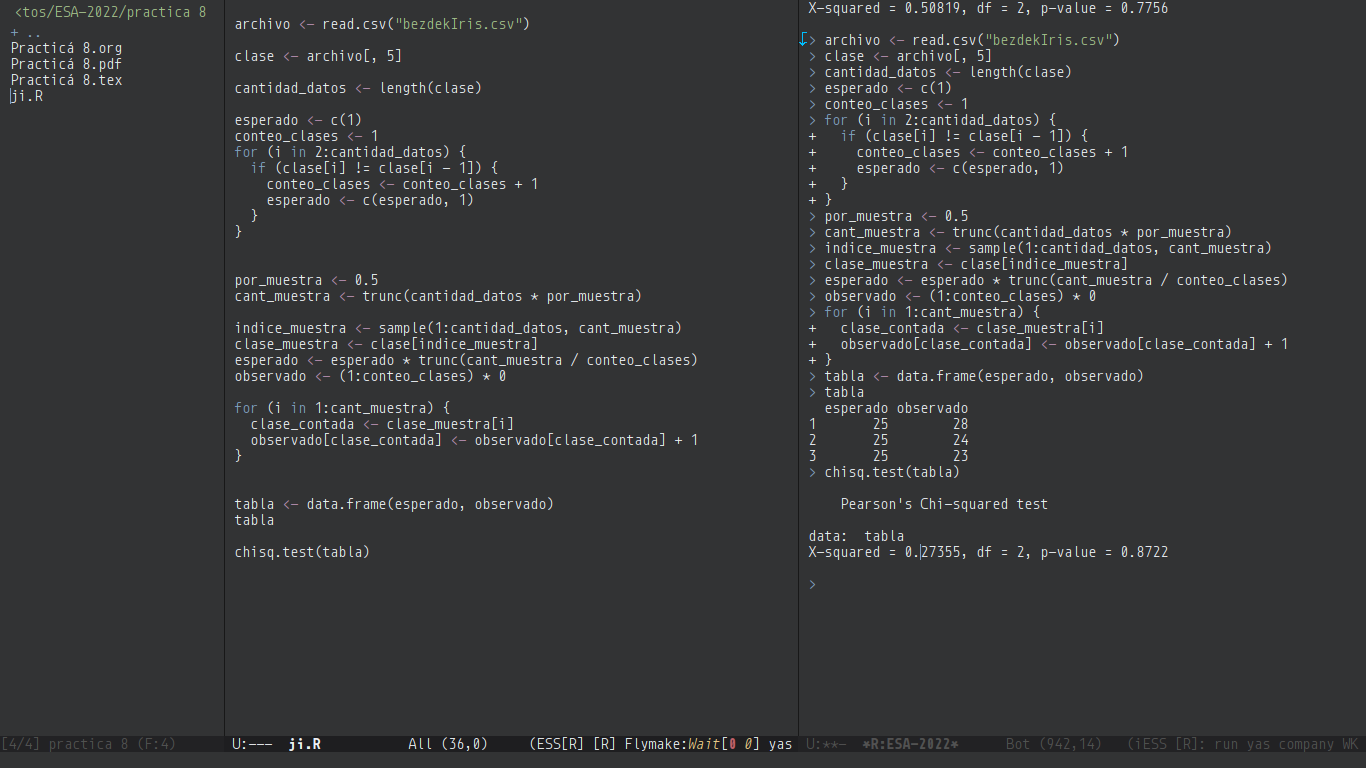
\includegraphics[width=.9\linewidth]{img/1.png}
\caption{p-value = 0.8722}
\end{figure}

\begin{figure}[htbp]
\centering
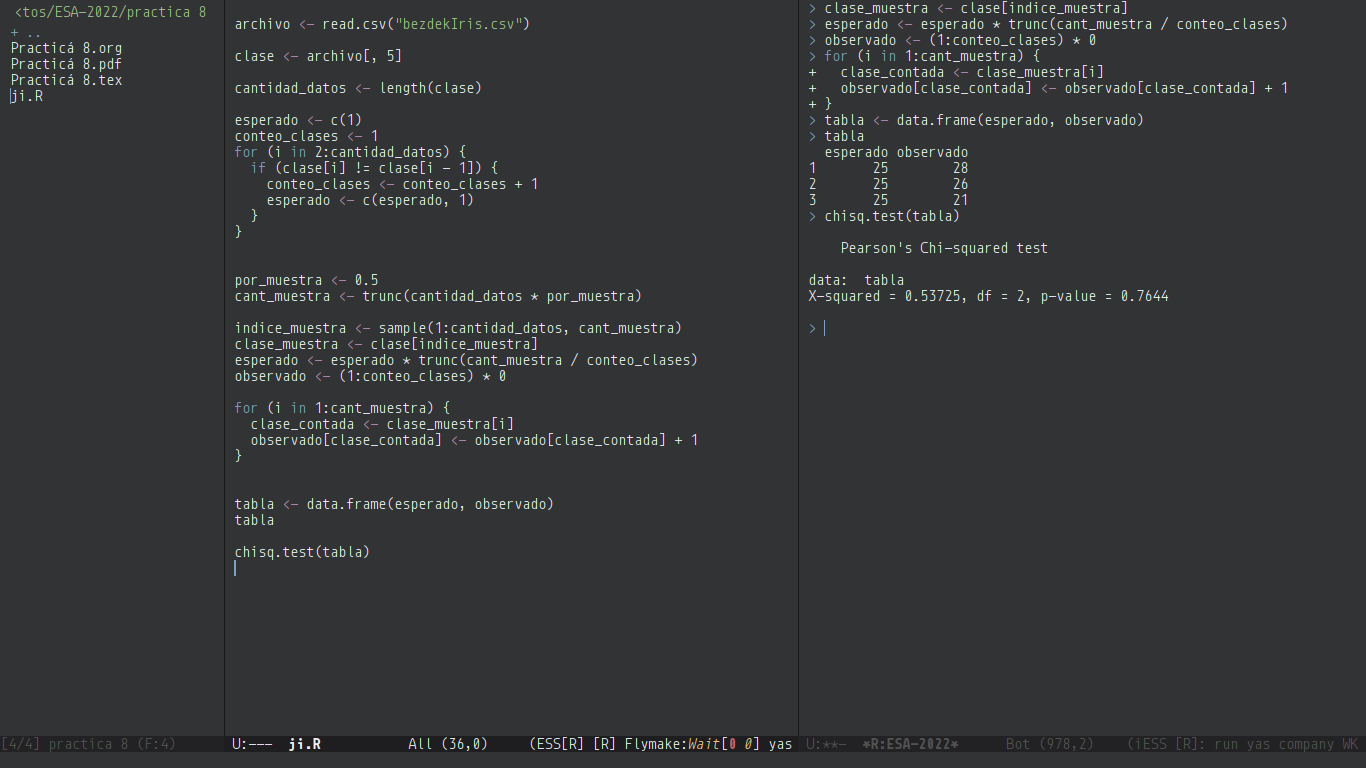
\includegraphics[width=.9\linewidth]{img/2.png}
\caption{p-value = 0.7644}
\end{figure}

\begin{figure}[htbp]
\centering
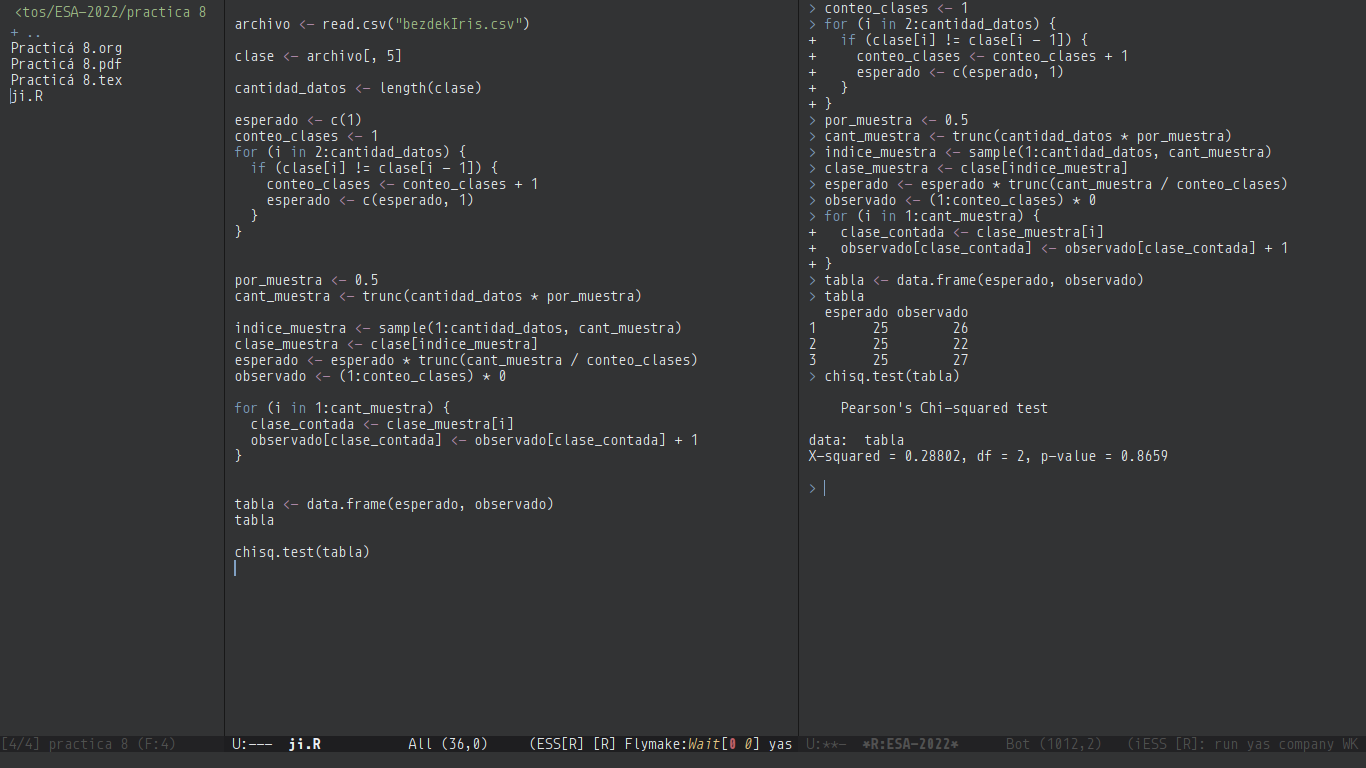
\includegraphics[width=.9\linewidth]{img/3.png}
\caption{p-value = 0.8659}
\end{figure}

\pagebreak

\section*{Código}
\label{sec:org0973077}
\lstinputlisting{./ji.R}
\end{document}
